\documentclass[11pt]{article}
\title{Meccano triangles}
\author{https://github.com/heptagons/meccano/nest}
\date{}

\newfam\bbbfam
\font\bbbten=msbm10
\font\bbbseven=msbm7
\font\bbbfive=msbm5
\textfont\bbbfam=\bbbten
\scriptfont\bbbfam=\bbbseven
\scriptscriptfont\bbbfam=\bbbfive
\def\bbb{\fam=\bbbfam}

\usepackage{../../meccano}
\begin{document}

\maketitle
\begin{abstract}
We construct meccano triangles. Basic triangles has the three sides as integers and calculate the internal diagonal distances.
Such diagonals then are used as the new side of more complicated triangles and then again we
calculate new distances formed and so on. Eventually we expect to
find certain angles joining the triangles which can be used to construct regular polygons or more figures.
\end{abstract}

\section{Triangle $(a,b,c)$}
A triangle $(a,b,c)$ has the tree integer sides $a$, $b$ and $c$ where $a, b, c \in \bbb N$.
To avoid repetitions and get only valid triangles, we consider only the cases:
\begin{align}
a &\ge b \ge c\\
a &< b + c
\end{align}
We calculate the three angles cosines. The three cosines are rationals:
\begin{align}
\cos{A} &= \frac{b^2 + c^2 - a^2}{2bc} &\in \bbb Q\\
\cos{B} &= \frac{c^2 + a^2 - b^2}{2ca} &\in \bbb Q\\
\cos{C} &= \frac{a^2 + b^2 - c^2}{2ab} &\in \bbb Q
\end{align}

\subsection{Triangle $(a,b,c)$ diagonals}

To calculate the diagonals we use the law of cosines.
With the $\cos{A}$ we can calculate every diagonal $\overline{b_mc_n}$ with:
\begin{align}
\overline{b_mc_n} &= \sqrt{m^2 + n^2 - 2mn\cos{A}}\\
       &= \sqrt{m^2 + n^2 - 2mn\frac{b^2 + c^2 - a^2}{2bc}}\\
       &= \frac{\sqrt{b^2c^2(m^2 + n^2)-bcmn(b^2 + c^2 - a^2)}}{bc} &\in \bbb A
\end{align}
where $1 \le m \le b$, $1 \le n \le c$ and $m - n \ge 0$. Similarly:
\begin{align}
\overline{c_ma_n} &= \frac{\sqrt{c^2a^2(m^2 + n^2)-camn(c^2 + a^2 - b^2)}}{ac} &\in \bbb A\\
\overline{a_mb_n} &= \frac{\sqrt{a^2b^2(m^2 + n^2)-abmn(a^2 + b^2 - c^2)}}{ab} &\in \bbb A
\end{align}
The diagonals are algebraic of the form $\frac{y\sqrt{z}}{x}$.

\subsection{Example triangle (7,6,5)}

\begin{figure}[htp]
\centering
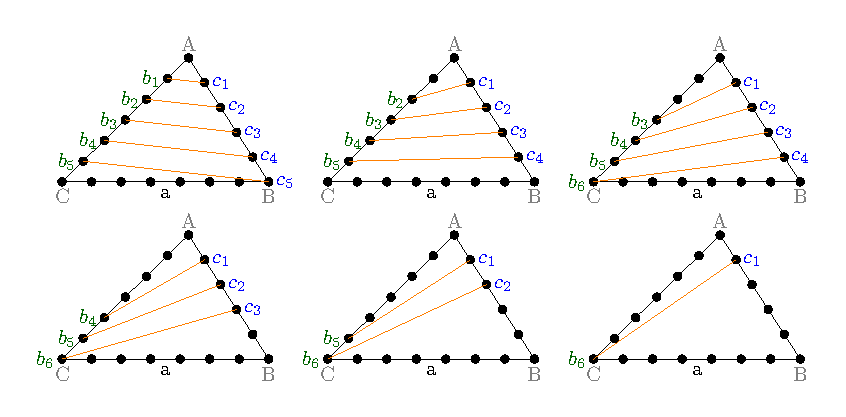
\includegraphics[scale=1]{t765bc}
\caption{Triangle $(7,6,5)$ $b_mc_n$ diagonals ($m \ge n$).
For top to bottom and left to right we have six groups of diagonals.
Each group is defined by $m$ and $n$ indices difference:
$m - n = 0$, $m - n = 1$, ... $m - n = 5$.
}
\label{t765bc}
\end{figure}

\begin{figure}[htp]
\centering
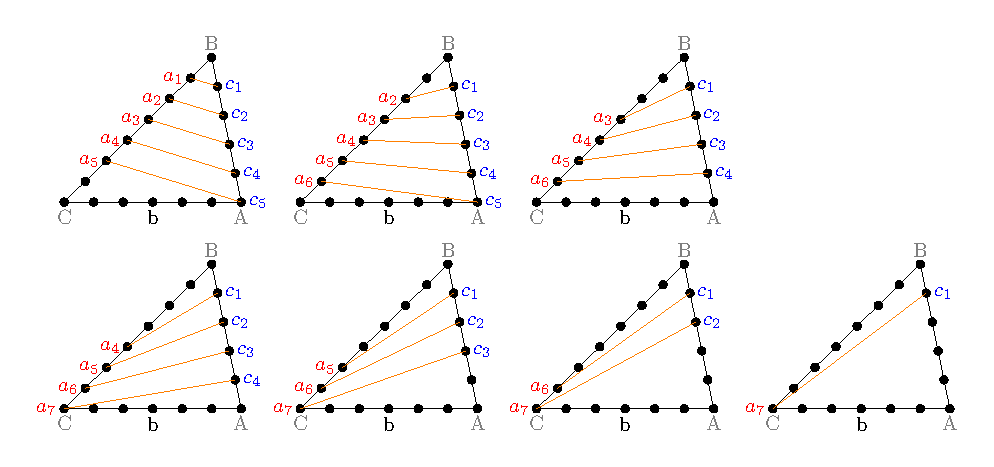
\includegraphics[scale=1]{t765ac}
\caption{Triangle $(7,6,5)$, $a_mc_n$ diagonals ($m \ge n$).
We have also six group. But here we found diagonals repetead already
found in previous figure. Diagonals repeated are all including $a_7$ points.
}
\label{t765ac}
\end{figure}

\begin{figure}[htp]
\centering
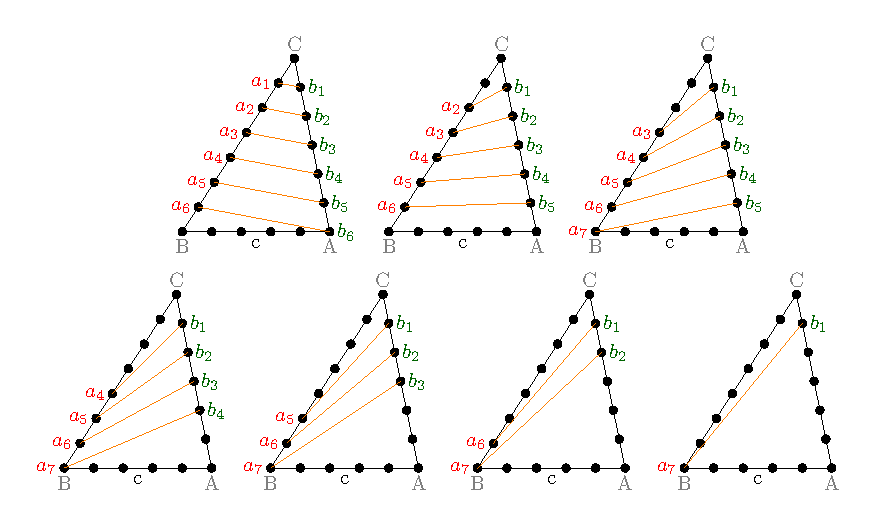
\includegraphics[scale=1]{t765ab}
\caption{Triangle $(7,6,5)$, $a_mb_n$ diagonals ($m \ge n$).
Here we have diagonals repeteated already in previous figure.
Using matrices we can reject such diagonals rejecting matrices columns.
}
\label{t765ab}
\end{figure}

\newcommand\five{\colorbox{green}{$5$}}

Figure \ref{t765bc} show triangle $(7,6,5)$ diagonals $b_mc_n$ for vertex $A$. For this figure we calculate
the values and form a matrix. Empty cells are reflections:
\begin{equation}\label{eq:appendrow}
\left(\begin{array}{cccccc}
	\frac{2\sqrt{10}}{5} & \frac{\sqrt{105}}{5} & \frac{2\sqrt{55}}{5} & \frac{\sqrt{385}}{5} & 2\sqrt{6} & \frac{\sqrt{865}}{5} \\
	& \frac{4\sqrt{10}}{5} & \frac{\sqrt{265}}{5} & \frac{2\sqrt{105}}{5} & \five & \frac{4\sqrt{55}}{5} \\
	& & \frac{6\sqrt{10}}{5} & \frac{\sqrt{505}}{5} & 2\sqrt{7} & \frac{3\sqrt{105}}{5}\\
	& & & \frac{8\sqrt{10}}{5} & \sqrt{33} & \frac{2\sqrt{265}}{5}\\
	& & & & 2\sqrt{10} & \boxed{7} \\
\end{array}\right)
\end{equation}

Figure \ref{t765ac} show triangle $(7,6,5)$ diagonals $a_mc_n$ for vertex $B$. For this figure we calculate
the values for a second matrix. Values at column 7 (at the right of separator $|$) are repeated and already in previous matrix.
Empty cells are reflections.
\begin{equation}\label{eq:appendrow}
\left(\begin{array}{cccccccc}
	\frac{4\sqrt{70}}{35} & \frac{3\sqrt{385}}{35} & \frac{2\sqrt{2065}}{35} & \frac{\sqrt{15505}}{35} & \frac{12\sqrt{7}}{7} & \frac{\sqrt{37345}}{35} & | & \frac{2\sqrt{265}}{5}\\
	& \frac{8\sqrt{70}}{35} & \frac{\sqrt{7945}}{35} & \frac{6\sqrt{385}}{35} & \frac{\sqrt{889}}{7} & \frac{4\sqrt{2065}}{35} & | & \frac{3\sqrt{105}}{5} \\
	& & \frac{12\sqrt{70}}{35} & \frac{\sqrt{14665}}{35} & \frac{2\sqrt{217}}{7} & \frac{9\sqrt{385}}{35} & | & \frac{4\sqrt{55}}{5}\\
	& & & \frac{16\sqrt{70}}{35} & \frac{3\sqrt{105}}{7} & \frac{2\sqrt{7945}}{35} & | & \frac{\sqrt{865}}{5}\\
	& & & & \frac{4\sqrt{70}}{7} & \frac{\sqrt{1393}}{7} & | & \boxed{6}\\
\end{array}\right)
\end{equation}

Figure \ref{t765ab} show triangle $(7,6,5)$ diagonals $a_mb_n$ for vertex $C$. For this figure we calculate
the values for a third matrix. Values at columns 6 and 7 (at the right of separator $|$) 
are repeated and already in previous matrices.
\begin{equation}\label{eq:appendrow}
\left(\begin{array}{cccccccc}
	\frac{2\sqrt7}7 & \frac{\sqrt{105}}7 & \frac{2\sqrt{70}}7 & \frac{\sqrt{553}}7 & \frac{2\sqrt{231}}7 & | &  \frac{\sqrt{1393}}7 & 2\sqrt{10} \\
	 & \frac{4\sqrt7}7 & \frac{\sqrt{217}}7 & \frac{2\sqrt{105}}7 & \frac{\sqrt{721}}7 & | &  \frac{4\sqrt{70}}7 & \sqrt{33} \\
	 & & \frac{6\sqrt7}7 & \frac{\sqrt{385}}7 & \frac{2\sqrt{154}}7 & | &  \frac{3\sqrt{105}}7 & 2\sqrt{7} \\
	 & & & \frac{8\sqrt7}7 & \frac{\sqrt{609}}7 & | &  \frac{2\sqrt{217}}7 & \five \\
	 & & & & \frac{10\sqrt7}7 & | &  \frac{\sqrt{889}}7 & 2\sqrt{6} \\
	 & & & & & | & \frac{12\sqrt7}7 & \boxed{5} \\
\end{array}\right)
\end{equation}

\section{Triangles$(\sqrt{a},b,c)$}

Triangles$(\sqrt{a},b,c)$ have the tree sides $\sqrt{a}$, $b$ and $c$ so we have:
\begin{align}
a, b, c &\in \bbb N\\
\sqrt{a} &> b \ge c &\implies a  > b^2 \ge c^2 \\
\sqrt{a} &< b + c   &\implies a < (b + c)^2
\end{align}
We calculate the triangle cosines. $\cos{A}$ is rational but $\cos{B}$ and $\cos{C}$ are algebraic:
\begin{align}
\cos{A} &= \frac{b^2 + c^2 - (\sqrt{a})^2}{2bc} = \frac{b^2 + c^2 - a}{2bc} &\in \bbb{Q} \\
\cos{B} &= \frac{(\sqrt{a})^2 + c^2 - b^2}{2\sqrt{a}c} = \frac{(a + c^2 - b^2)\sqrt{a}}{2ac} &\in \bbb{A} \\
\cos{C} &= \frac{(\sqrt{a})^2 + b^2 - c^2}{2\sqrt{a}b} = \frac{(a + b^2 - c^2)\sqrt{a}}{2ab} &\in \bbb{A} 
\end{align}

\subsection{Triangle $(\sqrt{a},b,c)$ diagonals}

The only possible diagonals are for sides with integers, that is $\overline{b_mc_n}$. Using the law of cosines:
\begin{align}
\overline{b_mc_n} &= \sqrt{m^2 + n^2 - 2mn\cos{A}}\\
  &= \sqrt{m^2 + n^2 - 2mn\frac{b^2 + c^2 - a}{2bc}}\\
  &= \frac{\sqrt{b^2c^2(m^2 + n^2)-bcmn(b^2 + c^2 - a)}}{bc} &\in \bbb{A}
\end{align}
where $1 \le m \le b$, $1 \le n \le c$ and $m - n \ge 0$.

\subsection{Example triangles$(2\sqrt{6},b,c)$}

In this case $\sqrt{a} = 2\sqrt{6}$ so $a = 24$. Then $m = n = \{ 1,2,3,4 \}$ because $b^2 = c^2 = \{ 1,4,9,16\} < 24$.
We form a matrix with with the values $(b+c)^2$:
\begin {equation}\label{E:1}
(b_i + c_j)^2 =\bordermatrix{~ & b=1 & b=2 & b=3 & b=4 \cr
c=1 &  4 &  9 & 16 & 25 \cr    
c=2 &  9 & 16 & 25 & 36 \cr    
c=3 & 16 & 25 & 36 & 49 \cr    
c=4 & 25 & 36 & 49 & 64 \cr}
\end {equation}

Then we remove cells which don't fulfil condition $b \ge c$:
\begin {equation}\label{E:2}
(b_i + c_j)^2 =\bordermatrix{~ & b=1 & b=2 & b=3 & b=4 \cr
c=1 &  2 &  9 & 16 & 25 \cr    
c=2 & \times & 16 & 25 & 36 \cr    
c=3 & \times & \times & 36 & 49 \cr    
c=4 & \times & \times & \times & 64 \cr}
\end {equation}

Finally we remove cells which don't fulfil condition $a < (b+c)^2$:
\begin {equation}\label{E:3}
(b_i + c_j)^2 =\bordermatrix{~ & b=1 & b=2 & b=3 & b=4 \cr
c=1 & \times & \times & \times & 25 \cr    
c=2 & & \times & 25 & 36 \cr    
c=3 & & & 36 & 49 \cr    
c=4 & & & & 64 \cr}
\end {equation}
    
So only six triangles are valid:
\begin {equation}\label{E:4}
(2\sqrt{6},b,c) =\bordermatrix{~ & \cos{A} & \cos{B} & \cos{C} \cr
(2\sqrt{6},3,2) & -\frac{11}{12} & \frac{19\sqrt{6}}{48} & \frac{29\sqrt{6}}{72} \cr
(2\sqrt{6},3,3) & -\frac{1}{3}   & \frac{\sqrt{6}}{3}    & \frac{\sqrt{6}}{3}    \cr
(2\sqrt{6},4,1) & -\frac{7}{8}   & \frac{3\sqrt{6}}{8}   & \frac{13\sqrt{6}}{32} \cr
(2\sqrt{6},4,2) & -\frac{1}{4}   & \frac{\sqrt{6}}{4}    & \frac{3\sqrt{6}}{8}   \cr
(2\sqrt{6},4,3) &  \frac{1}{24}  & \frac{17\sqrt{6}}{72} & \frac{31\sqrt{6}}{96} \cr
(2\sqrt{6},4,4) &  \frac{1}{4}   & \frac{\sqrt{6}}{4}    & \frac{\sqrt{6}}{4}    \cr}
\end{equation}

data from \texttt{github.com/heptagons/meccano/nest/t\_test.go TestTslursA}

\section{Triangles$(a,\sqrt{b},c)$}

Triangles$(a,\sqrt{b},c)$ have the tree sides $a$, $\sqrt{b}$, $c$ where $a, b, c \in \bbb N$ and $b$ is squarefree. We have:
\begin{align}
a &> \sqrt{b} > c &\implies a^2 > b > c^2 \\
a &< \sqrt{b} + c &\implies (a-c)^2 < b
\end{align}
We calculate the triangle cosines. $\cos{A}$ is algebraic, $\cos{B}$ rational and $\cos{C}$ algebraic:
\begin{align}
\cos{A} &= \frac{b + c^2 - a^2}{2\sqrt{b}c} = \frac{(b + c^2 - a^2)\sqrt{b}}{2bc} &\in \bbb{A} \\
\cos{B} &= \frac{a^2 + c^2 - (\sqrt{b})^2}{2ac} = \frac{a^2 + c^2 - b}{2ac} &\in \bbb{Q} \\
\cos{C} &= \frac{a^2 + (\sqrt{b})^2 - c^2}{2a\sqrt{b}} = \frac{(a^2 + b - c^2)\sqrt{b}}{2ab} &\in \bbb{A} 
\end{align}

\subsection{Triangle $(a, \sqrt{b},c)$ diagonals}

The only possible diagonals are for sides with integers, that is $\overline{a_mc_n}$. Using the law of cosines:
\begin{align}
\overline{a_mc_n} &= \sqrt{m^2 + n^2 - 2mn\cos{B}}\\
  &= \sqrt{m^2 + n^2 - 2mn\frac{a^2 + c^2 - b}{2ac}}\\
  &= \frac{\sqrt{a^2c^2(m^2 + n^2)-acmn(a^2 + c^2 - b)}}{ac} &\in \bbb{A}
\end{align}
where $1 \le m \le a$, $1 \le n \le c$ and $m - n \ge 0$.

\subsection{Example triangles$(a,2\sqrt{6},c)$}

In this case $\sqrt{b} = 2\sqrt{6}$ so $b = 24$. Then $n = \{ 1,2,3,4 \}$ because $c^2 = \{ 1,4,9,16\} < 24$.
We form a matrix with with the values $(a-c)^2$ starting with $a=5$ to fulfil $a^2 > b$:
\begin {equation}\label{E:11}
(a_m - c_n)^2 =\bordermatrix{~ & a=5 & a=6 & a=7 & ...\cr
c=1 & 16 & 25 & 36 & ... \cr    
c=2 & 25 & 36 & 49 & ... \cr    
c=3 & 36 & 49 & 64 & ... \cr    
c=4 & 49 & 64 & 81 & ... \cr}
\end {equation}

We remove cells which don't fulfil condition $(a-c)^2 < b$:
\begin {equation}\label{E:12}
(a_m - c_n)^2 =\bordermatrix{~ & a=5 & a=6 & a=7 & ...\cr
c=1 & 16 & \times & \times & ... \cr    
c=2 & \times & \times & \times & ... \cr    
c=3 & \times & \times & \times & ... \cr    
c=4 & \times & \times & \times & ... \cr}
\end {equation}

So only one triangles are valid:
\begin {equation}\label{E:13}
(a,2\sqrt{6},c) =\bordermatrix{~ & \cos{A} & \cos{B} & \cos{C} \cr
(5,2\sqrt{6},1) & \frac{}{} & \frac{}{} & \frac{}{} \cr}
\end{equation}

data from \texttt{github.com/heptagons/meccano/nest/t\_test.go TestTslursB}


\section{Triangles$(a,b,\sqrt{c})$}

Triangles$(a,b,\sqrt{c})$ have the tree sides $a$, $b$, $\sqrt{c}$ where $a, b, c \in \bbb N$ and $c$ is squarefree. We have:
\begin{align}
a &\ge b > \sqrt{c} &\implies a^2 \ge b^2 > c \\
a &< b + \sqrt{c} &\implies (a-b)^2 < c
\end{align}
We calculate the triangle cosines. $\cos{A}$ and $\cos{B}$ are algebraic and $\cos{C}$ rational:
\begin{align}
\cos{A} &= \frac{b^2 + c - a^2}{2b\sqrt{c}} = \frac{(b^2 + c - a^2)\sqrt{c}}{2bc} &\in \bbb{A} \\
\cos{B} &= \frac{a^2 + c - b^2}{2a\sqrt{c}} = \frac{(a^2 + c - b^2)\sqrt{c}}{2ac} &\in \bbb{A} \\
\cos{C} &= \frac{a^2 + b^2 - (\sqrt{c})^2}{2ab} = \frac{a^2 + b^2 - c}{2ab} &\in \bbb{Q} 
\end{align}

\subsection{Triangle $(a, b, \sqrt{c})$ diagonals}

The only possible diagonals are for sides with integers, that is $\overline{a_mb_n}$. Using the law of cosines:
\begin{align}
\overline{a_mb_n} &= \sqrt{m^2 + n^2 - 2mn\cos{C}}\\
  &= \sqrt{m^2 + n^2 - 2mn\frac{a^2 + b^2 - c}{2ab}}\\
  &= \frac{\sqrt{a^2b^2(m^2 + n^2)-acmn(a^2 + b^2 - c)}}{ab} &\in \bbb{A}
\end{align}
where $1 \le m < a$, $1 \le n < b$ and $m - n \ge 0$.

\subsection{Example triangles$(a,b,2\sqrt{6})$}

In this case $\sqrt{c} = 2\sqrt{6}$ so $c = 24$. 
We form a matrix with with the values $(a-b)^2$ starting with $a=5$ and $b=5$ to fulfil $a^2 \ge b^2 > c$:
\begin {equation}\label{E:21}
(a_m - b_n)^2 =\bordermatrix{~ & a=5 & a=6 & a=7 & a=8 & a=9 & a=10 & a=11 & a=12 & \hdots\cr
b=5  & 0 & 1 & 4 &  9 & 16 & 25 & 36 & 49 & \hdots \cr    
b=6  &   & 0 & 1 &  4 &  9 & 16 & 25 & 36 & \hdots \cr    
b=7  &   &   & 0 &  1 &  4 &  9 & 16 & 25 & \hdots \cr    
b=8  &   &   &   &  0 &  1 &  4 &  9 & 16 & \hdots \cr    
b=9  &   &   &   &    &  0 &  1 &  4 &  9 & \hdots \cr    
b=10 &   &   &   &    &    &  0 &  1 &  4 & \hdots \cr    
\vdots & \vdots & \vdots & \vdots & \vdots & \vdots & \vdots & \vdots & \vdots & \ddots \cr}
\end {equation}

We remove cells which don't fulfil condition $(a-b)^2 < c$, here $c=24$:
\begin {equation}\label{E:21}
(a_m - b_n)^2 =\bordermatrix{~ & a=5 & a=6 & a=7 & a=8 & a=9 & a=10 & a=11 & a=12 & \hdots\cr
b=5  & 0 & 1 & 4 &  9 & 16 & \times & \times & \times & \hdots \cr    
b=6  &   & 0 & 1 &  4 &  9 & 16 & \times & \times & \hdots \cr    
b=7  &   &   & 0 &  1 &  4 &  9 & 16 & \times & \hdots \cr    
b=8  &   &   &   &  0 &  1 &  4 &  9 & 16 & \hdots \cr    
b=9  &   &   &   &    &  0 &  1 &  4 &  9 & \hdots \cr    
b=10 &   &   &   &    &    &  0 &  1 &  4 & \hdots \cr    
\vdots & \vdots & \vdots & \vdots & \vdots & \vdots & \vdots & \vdots & \vdots & \ddots \cr}
\end {equation}


\end{document}